\documentclass{article}
\usepackage{tikz}
\usetikzlibrary{positioning, arrows.meta}

\begin{document}

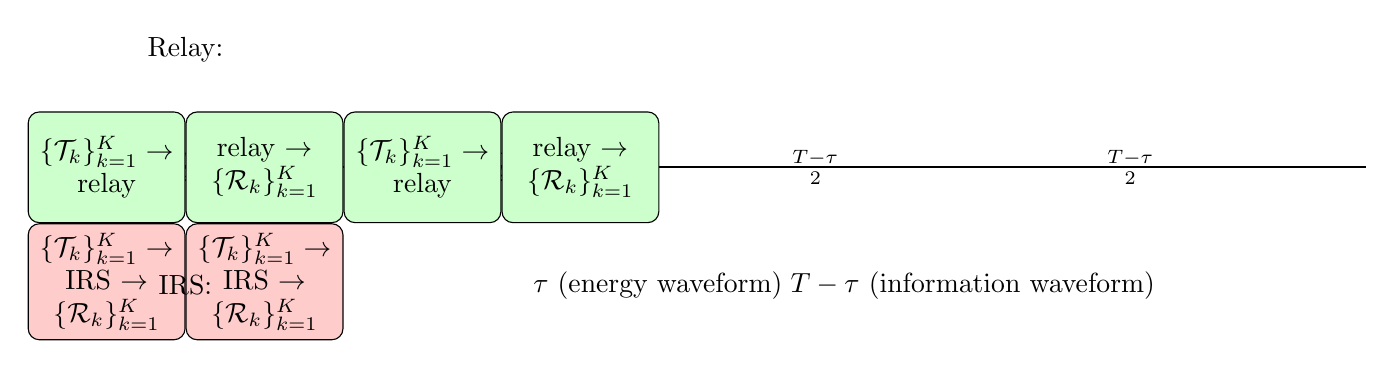
\begin{tikzpicture}[node distance=0pt, auto,
    block/.style={rectangle, draw, fill=green!20, 
                  text width=5em, text centered, rounded corners, minimum height=4em},
    block2/.style={rectangle, draw, fill=red!20, 
                  text width=5em, text centered, rounded corners, minimum height=4em},
    line/.style={draw, -Latex}]

% Draw the timeline
\draw[thick] (0,0) -- (16,0);

% Labels for the timeline
\node at (1,0) {$\frac{\tau}{2}$};
\node at (5,0) {$\frac{\tau}{2}$};
\node at (9,0) {$\frac{T-\tau}{2}$};
\node at (13,0) {$\frac{T-\tau}{2}$};

% Relay nodes
\node[block] (relay1) {$\{\mathcal{T}_k\}_{k=1}^K \rightarrow$ relay};
\node[block] (relay2) [right=of relay1] {relay $\rightarrow \{\mathcal{R}_k\}_{k=1}^K$};
\node[block] (relay3) [right=of relay2] {$\{\mathcal{T}_k\}_{k=1}^K \rightarrow$ relay};
\node[block] (relay4) [right=of relay3] {relay $\rightarrow \{\mathcal{R}_k\}_{k=1}^K$};

% IRS nodes
\node[block2] (irs1) [below=of relay1] {$\{\mathcal{T}_k\}_{k=1}^K \rightarrow$ IRS $\rightarrow \{\mathcal{R}_k\}_{k=1}^K$};
\node[block2] (irs2) [below=of relay2] {$\{\mathcal{T}_k\}_{k=1}^K \rightarrow$ IRS $\rightarrow \{\mathcal{R}_k\}_{k=1}^K$};

% Labels for the IRS and Relay
\node at (1,-1.5) {IRS:};
\node at (1,1.5) {Relay:};

% Labels for the waveforms
\node at (7,-1.5) {$\tau$ (energy waveform)};
\node at (11,-1.5) {$T-\tau$ (information waveform)};

\end{tikzpicture}

\end{document}